
\documentclass[review,12pt,authoryear]{elsarticle}

%% The amssymb package provides various useful mathematical symbols
\usepackage{amssymb}
%% The amsthm package provides extended theorem environments
%% \usepackage{amsthm}

%% The lineno packages adds line numbers. Start line numbering with
%% \begin{linenumbers}, end it with \end{linenumbers}. Or switch it on
%% for the whole article with \linenumbers.
\usepackage{lineno}

% for adjusting table width automatically
\usepackage{adjustbox}
\usepackage{tabulary, ragged2e}
\usepackage{booktabs}

% Below is Elseviers requirements - they are similar to most articles and a good point of reference when writting scientific articles or analyses in general.
%1.Full Length Article A full-length article should be a substantial and in-depth research study regarding a particular state of issue through several techniques or approaches. 
% The main text should be approximately 6,000 words in length, but it should not exceed 8,000 words (excluding abstract, references, tables, figures, and appendices).
%A maximum of 250 words abstract and up to 10 displayed items (figures and tables) is allowed. A full-length article should include an Introduction,
%Materials and methods, Results, Discussion, Conclusions, and References, which can be accompanied by Supplementary material.

\begin{document}
\begin{linenumbers}
\begin{frontmatter}

%%%%%%%%%%%%%%%%%%%%%%%%%%%%%%%%%%%%%%%%%%
%%              Start Matter            %%
%%%%%%%%%%%%%%%%%%%%%%%%%%%%%%%%%%%%%%%%%%

%% Title, authors and addresses

%% use the tnoteref command within \title for footnotes;
%% use the tnotetext command for theassociated footnote;
%% use the fnref command within \author or \affiliation for footnotes;
%% use the fntext command for theassociated footnote;
%% use the corref command within \author for corresponding author footnotes;
%% use the cortext command for theassociated footnote;
%% use the ead command for the email address,
%% and the form \ead[url] for the home page:

%% \title{Title\tnoteref{label1}}
\title{???Grape Quality and its Link to Regional Differences in the Australian Winegrowing Industry}
% Regional differences in Australian winegrowing (Quality)?

%% \tnotetext[label1]{}
%% \author{Name\corref{cor1}\fnref{label2}}
%% \ead{email address}
%% \ead[url]{home page}
%% \fntext[label2]{}
%% \cortext[cor1]{}
%% \affiliation{organization={},
%%            addressline={}, 
%%            city={},
%%            postcode={}, 
%%            state={},
%%            country={}}
%% \fntext[label3]{}

%% use optional labels to link authors explicitly to addresses:
%% \author[label1,label2]{}
%% \affiliation[label1]{organization={},
%%             addressline={},
%%             city={},
%%             postcode={},
%%             state={},
%%             country={}}
%%
%% \affiliation[label2]{organization={},
%%             addressline={},
%%             city={},
%%             postcode={},
%%             state={},
%%             country={}}
%\affiliation[label1]{organization={QUT},
%  addressline={},
%  city={},
%  postcode={},
%  state={QLD},
%  country={}}
%\affiliation[label2]{organization={AWRI},
%  addressline={},
%  city={},
%  postcode={},
%  state={SA},
%  country={}}
%\affiliation[label3]{organization={Food Agility CRC},
%  addressline={},
%  city={},
%  postcode={},
%  state={Vic},
%  country={}}
\author[label1,label2,label3]{Author}
\date{02/08/2023}

\begin{abstract}
\end{abstract}
%%Graphical abstract`
%\begin{graphicalabstract}
 % \includegraphics{graphical_abstract.jpeg}
%\end{graphicalabstract}'

%\begin{keyword}
%% keywords here, in the form: keyword \sep keyword
%Keyword one \sep{} keyword two
%% PACS codes here, in the form: \PACS code \sep code
%\PACS{} 0000 \sep{} 1111
%% MSC codes here, in the form: \MSC code \sep code
%% or \MSC[2008] code \sep code (2000 is the default)
%\MSC{} 0000 \sep{} 1111
%\end{keyword}
%%Research highlights
\begin{highlights}
  \item ???
  \item ???
  \item ????
  \item ????
\end{highlights}
\end{frontmatter}

%%%%%%%%%%%%%%%%%%%%%%%%%%%%%%%%%%%%%%%%%%
%%                main text             %%
%%%%%%%%%%%%%%%%%%%%%%%%%%%%%%%%%%%%%%%%%%

\section{Introduction}

% You obviously have no leading question for this paper, and although you do a good job at creating accurate models; it is more important that the research is asking a good question. A cool question as Kate puts it.
%
% The questions I put forward to you are:
%
%   How do winegrowing regions differ?
%   Why is a region different?
%   How do regional differences affect winegrowing?
%   What differences are important between winegrowing regions?
%   
%

\if{false}

We classify regions to find the most prominent and well-defined relationships to regions.
We examine the variables that are the most decisive in determining region.
We compare the similarities and differences of these regions
- within the analysis and
- within the literature (also in their definition and history)

We examine the similarity between these classifications and the variables that are significant in classifying profitable vs not.
How do regional changes affect that. What is similar and what is different.

We can link these contributing factors back to the baselines - at least anecdotally, or in an unpublished section. This will be good for the thesis.

\fi

%%%%%%%%%%%%%%%%%%%%%%%%%%%%%%%%%%%%%
The Australian wine-growing industry is a rich and diverse landscape that is separated into multiple Geographical Indicator Regions. Each region describing unique reputations, qualities and varietals of wine produced there. While a great deal has been done regarding individual regional properties and traits, there has been little statistical insight into broader regional comparisons; due to a lack of cross-regional and in-depth data sources \citep{keithjonesAustralianWineIndustry2002,knightFirmResourcesDevelopment2019}. In this study we use Classification Trees to compare regional differences and how these differences relate to sustainable practices. 
\newline
A vineyard's region predetermines several physical parameters, such as: climate, geology and soil; making location a widely considered key determinant of grape yield and quality \citep{abbalDecisionSupportSystem2016,agostaRegionalClimateVariability2012,fragaMultivariateClusteringViticultural2017}. 
%
%This analysis addresses the knowledge gap regarding the effectiveness of regional level strategies employed in the wine industry and their relation to grape quality.
% What the hell is a regional strategy
% And how do you define, or know what trategy each region is using?
%
Through the use of classification trees this study aims to highlight the key differences in sustainable practices at a regional level and how these practices relate to the different grades of grape quality.

% This does not really address what the methods are - aside from classisifcation trees in the most vague sense.
% What are the results briefly? why should someone read this article?
% What is interesting - what will be discussed in the article with regard to these results? What makes me want to read the article?
% And what is the take away point of the article? If I cant be bothered to read this article, what piece of knowledge can you leave mewiwth that I could recommend the article to someone else with?

\if{false}
\begin{figure}
    \includegraphics{violinplot.pdf}
    \caption{Violin plots of GI Region and Year coefficients for each model.}\label{fig:violin}
    \end{figure}
  %
\fi{}

\section{Methods}

% As with the previous paper, put the models up front it is very unclear what you have created - and less clear to understand it if there is no way to reference to it.

\subsection{Data}

% 6091 samples - total
% 58 regions
% 10 years

% 853 with reported profits
% 46 regions
% reported since 2018
Data used in this analysis were obtained from Sustainable Winegrowing Australia. Australia's national wine industry sustainability program, which aims to facilitate grape-growers and winemakers in demonstrating and improving their sustainability \citep{swaSustainableWingrowingAustralia2022}. Data recorded by the SWA is entered manually by winegrowers using a web based interface tool. A total of 6091 observations were collected from 2012 to 2022. Each observation contained 23 variables reflecting a vineyards account for the given year (see Table \ref{tab:vars}).
\par
\begin{table}[] 
  \label{tab:vars}
  \caption{Summary of variables used in the analysis. The recorded column indicate values that were either greater than zero or that were not missing.}\label{tab:summary}
  \begin{tabular}{@{}ccccl@{}}
    \toprule
    \textbf{Variable} & \textbf{Units} & \textbf{Recorded} & \textbf{\begin{tabular}[c]{@{}c@{}}Number of\\ Classes\end{tabular}} &  \\ \midrule
    Water Used & Mega Litres & 5846 &  &  \\
    Diesel & Litres & 5585 &  &  \\
    Biodiesel & Litres & 25 &  &  \\
    LPG & Litres & 958 &  &  \\
    Herbicide Spray & Times per year & 2026 &  &  \\
    Year & Class & 6091 & 10 &  \\
    Disease & Class & 6091 & 2 &  \\
    Region & Class & 6091 & 58 &  \\
    Solar & Kilowatt Hours & 622 &  &  \\
    Irrigation Type & Class & 6091 & 20 &  \\
    Petrol & Litres & 4309 &  &  \\
    Slashing & Times per year & 2290 &  &  \\
    Yield & Tonnes & 5935 &  &  \\
    Irrigation Energy & Class & 6091 & 16 &  \\
    Area Harvested & Hectares & 6091 &  &  \\
    Electricity & Kilowatt Hours & 1015 &  &  \\
    Insecticide Spray & Times per year & 1092 &  &  \\
    Fertiliser & \begin{tabular}[c]{@{}c@{}}Kilograms \\ of Nitrogen\end{tabular} & 795 &  &  \\
    Fungicide Spray & Times per year & 2260 &  &  \\
    Cover Crop & Class & 6091 & 32 &  \\
    Water Type & Class & 6091 & 39 &  \\
    Profit & AUD & 853 &  &  \\
    Operating Costs & AUD & 853 &  &  \\ \bottomrule
    \end{tabular}
\end{table}

The data originally contained only two multiclass variables: year and region. Variables that measured the same metric from different sources (such as water collected from rivers versus water from dams) were converted into multiclass variables representing the source. The total amount used from these variables was retained as a separate variable. Occurrences of multiple sources were defined as separate classes. As harvest does not run by calendar year, years are in financial years. Region represents one of the 65 Geographical Indicator Regions (GI Region) used to describe different unique localised traits of vineyards across Australia \citep{hallidayAustralianWineEncyclopedia2009,oliverReviewSoilPhysical2013,soarClimateDriversRed2008}. Each region is explicitly defined under the Wine Australia Corporation Act of 1980 \citep{attorney-generalsdepartmentWineAustraliaCorporation2010}. Profit was also used as a binary variable, depicting whether a vineyard was profitable or not.
\par
%
% Mention one-hot-encoding.
%

%
% How deep into the classes do we go?
%
\subsection{XGBoosted Trees}
XGBoosted (eXtreme Gradient Boosting) trees were created using the XGBoost library \citep{chenXGBoostScalableTree2016} in the Python Programming language \citep{g.vanrossumPythonTutorialTechnical1995}. They were chosen for this analysis as they provide both a high predictive performance and ability to effectively capture complex relationships. An XGBoosted tree was created for each variable to show how they interacted. Each tree included all but the economic variables (profit and operating cost), which were only included once as predicted variables.
\par
Following Chen and Guestrin \citep{chenXGBoostScalableTree2016}, XGboosted trees predict a value $y_i$ from the input $x_i$. The method of prediction is achieved through a tree ensemble model, using $K$ additive functions to predict the output. 

\begin{equation}
  \hat{y_i}=\phi(x_i)=\sum_{k=1}^{K}{f_{K}(x_{i})}, f_{K}\in \mathcal{F},
\end{equation}

where each function $f_K$ is a classification or regression tree, such that all functions are in the set of all decision trees $\mathcal{F}$, defined by ${f(x) = \omega_{q(x)}}(q : \mathbb{R}^m \rightarrow T, \omega \in \mathbb{R}^T)$. Where, $f_K$ corresponds to an independent tree structure $q$ of $\omega$ weights. Each tree has $T$ leaves, which contain a continuous score, represented by $\omega_i$ for the i-th leaf. The final prediction is determined by the sum of the score of the corresponding leaves, given  by $\omega$. The set of functions used by the tree is determined by minimising the regularised objective function, given by:

\begin{equation}\label{eqn:objective}
 \mathcal{L}(\phi)=\sum_i l(\hat{y_i}, y_i^{t-1} + f_t(x_i)) + \sum_k \Omega (f_K).
\end{equation}

The difference between the prediction and actual variable is a convex loss function $l$. To optimise $l$, the difference is calculated for the i-th instance at the t-th iteration. The function $f_t$ is selected according to which value minimises (\ref{eqn:objective}). The model complexity is penalised by the function $\Omega$, this acts to smooth weights in an attempt to prevent over fitting.
\par
As predictions are made using additive tree functions, XGboosted trees can be used for classification and regression. Due to the mixture of continuous, binary and multiclass variables in this analysis, both classification and regression trees were created. The difference between the trees created for this analysis was the objective function used. XGBoosted regression trees were created for continuous variables, using the root-mean-square as the objective function. Binary class variables utilised the logistic loss function as the objective. And, Multiclass variable used the soft max function. All objective functions are defined within the SKlearn library \citep{sklearn_api}, linked via an API to the XGBoost library \citep{chenXGBoostScalableTree2016}.
\par
Chen and Guestrin \citep{chenXGBoostScalableTree2016} further illustrate, using Taylor expansions, that for a fixed structure $q(x)$ the optimal weight $\omega^*_j$ for a leaf $j$ can be derived. Furthermore, they show the loss reduction after the split is given by the function:

\begin{equation} \label{eqn:enumerate}
\mathcal{L}_{split} = {{1}\over{2}} \left[ 
  {{(\sum_{i\in I_L}g_i)^{2}}\over{\sum_{i\in I_L} h_i + \lambda}} +
  {{(\sum_{i\in I_R}g_i)^{2}}\over{\sum_{i\in I_R} h_i + \lambda}} -
  {{(\sum_{i\in I}{g_i})^{2}}\over{\sum_{i \in I} h_i + \lambda}} \right] - \gamma,
\end{equation}

with the tree structure defined using left $I_L$ and right $I_R$ instance sets of nodes, with $I = I_L \cup I_R$. Instead of enumerating all possible tree structures, a greedy algorithm iteratively adds branches to the tree minimising $ \mathcal{L}_{split} $ in (\ref{eqn:enumerate}). The frequency of a variable's occurrence within a tree is directly attributed to the minimisation of the objective function (or loss) through the minimisation of  $ \mathcal{L}_{split} $.
\par
The frequency of a variable appearing as a node within the ensemble was used as a measure of importance. This measure was chosen as it connected a variable to the minimisation of its associated objective function, translating the value into a simple count metric. Creating XGBoosted trees for each variable allowed the use of importance to show how strongly variables were associated with each other. The importance of predictor variables to economic variables was illustrated through the use of Sankey diagrams constructed using the Holoviews python library \citep{philipp_rudiger_2020_3904606}. Other variable's interconnectedness was demonstrated through the use of a chord diagram also created using Holoviews.
\par
Each variable utilised 80\% of the data to train the XGBoost ensemble, with 20\% reserved for testing and validation. Testing was done through the iterative minimisation of the respective objective function for the variables type. For continuous variables 20\% was used as testing data, minimising the root-mean-square function. The final model was validated using repeated k-fold cross validation for 10 folds, repeated 10 times.
 For  binary and multiclass variables data was split into 80\% training, 10\% testing and 10\% validation data. Due to class disparity in multiclass variables (most prominently in region) data was stratified into each subset at the same ratio of class occurrence. Validation was summarised through confusion matrices and their associated accuracy 
\par
The use of the XGBoost library incorporates regularisation techniques built into the software to mitigate over-fitting and enhance model generalisation. The further use of cross validated grid search functions allowed for the selection of better performing hyperparameters when selecting the final model. The performance measure for model selection was root-mean-square error for continuous variables. The receiver operator characteristic's area under the curve was used for category variables \citep{hanley1982meaning}. Multiclass variables utilised the one verse one approach to minimise sensitivity to class disparity \citep{ferriExperimentalComparisonPerformance2009,handSimpleGeneralisationArea2001}.

\subsection{Classification and Regression Trees}

Classification and Regression Trees were created for region, year, profit and operating cost. These models describe the partitions that are useful in predicting these variables; giving insight into the trees that make up the ensembles created by XGBoost. These trees were created using the rparts and caret packages \citep{kuhnBuildingPredictiveModels2008,terrytherneauRpartRecursivePartitioning2022} in the R statistical programming language \citep{rcoreteamLanguageEnvironmentStatistical2021}.
\par
Classification trees were validated using K-fold cross validation. Each model was validated using 10 folds, utilising a random selection of different samples ten separate times to validate each of the  classification trees. A summary confusion matrix was then constructed to show the class bias and overall accuracy of each tree.

\section{Results}


\subsection{Region}

\begin{figure}
  \resizebox{\textwidth}{!}{
  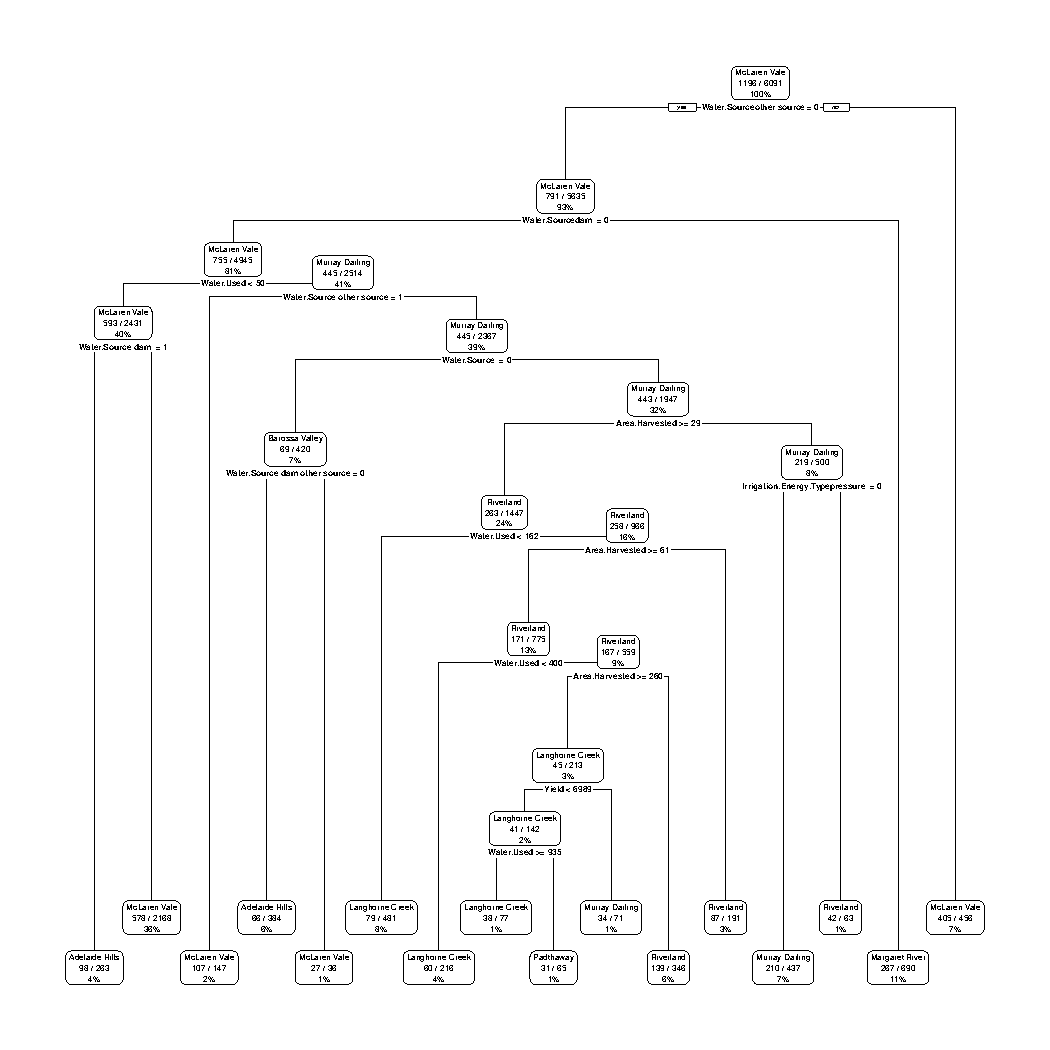
\includegraphics{region.pdf}}
  \caption{Decision tree predicting Region. Each node indicates the class predicted, and the proportion of elements agreeing with nodes partitioning, with the left direction indicating a yes to the nodes rule.}\label{fig:region_tree}
\end{figure}

\begin{figure}
  \resizebox{\textwidth}{!}{
  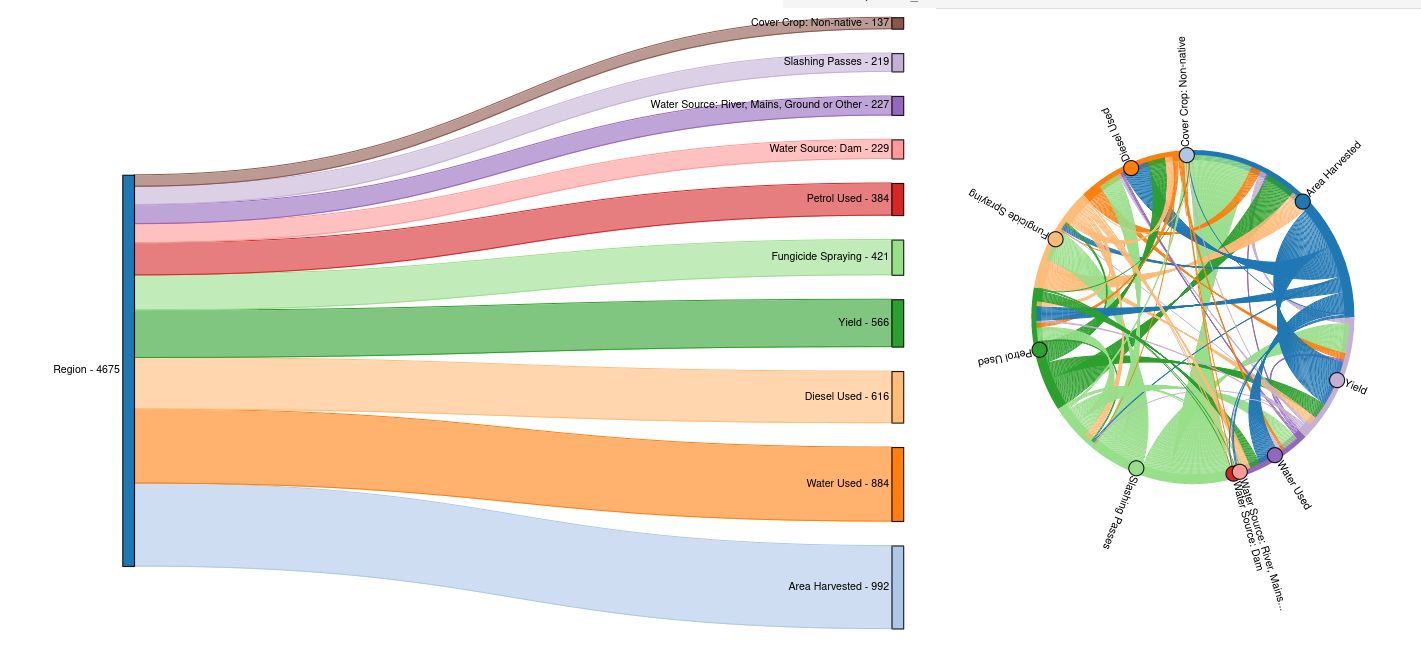
\includegraphics{region.png}}
  \caption{The left-hand side depicts the 10 most important variables in predicting Region using XGBoosted trees as a measure of node occurrence, using a Sankey diagram. The right-hand side depicts the interrelated importance of the ten predictor variables using a chord diagram.}\label{fig:region_sankey}
\end{figure}

\subsection{Year}

\begin{figure}
  \resizebox{\textwidth}{!}{
  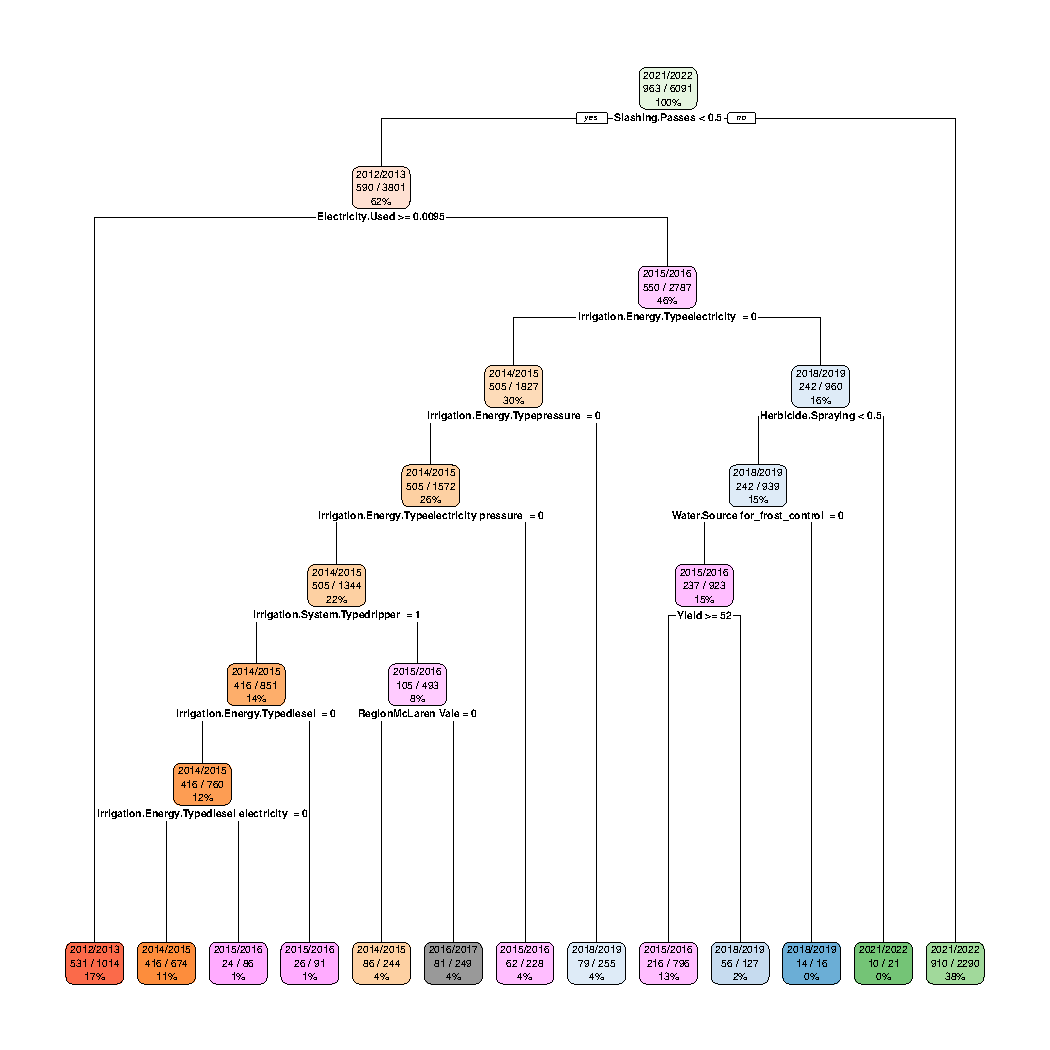
\includegraphics{year.pdf}}
  \caption{Decision tree predicting Year. Each node indicates the class predicted, and the proportion of elements agreeing with nodes partitioning, with the left direction indicating a yes to the nodes rule.}\label{fig:year_tree}
\end{figure}

\begin{figure}
  \resizebox{\textwidth}{!}{
  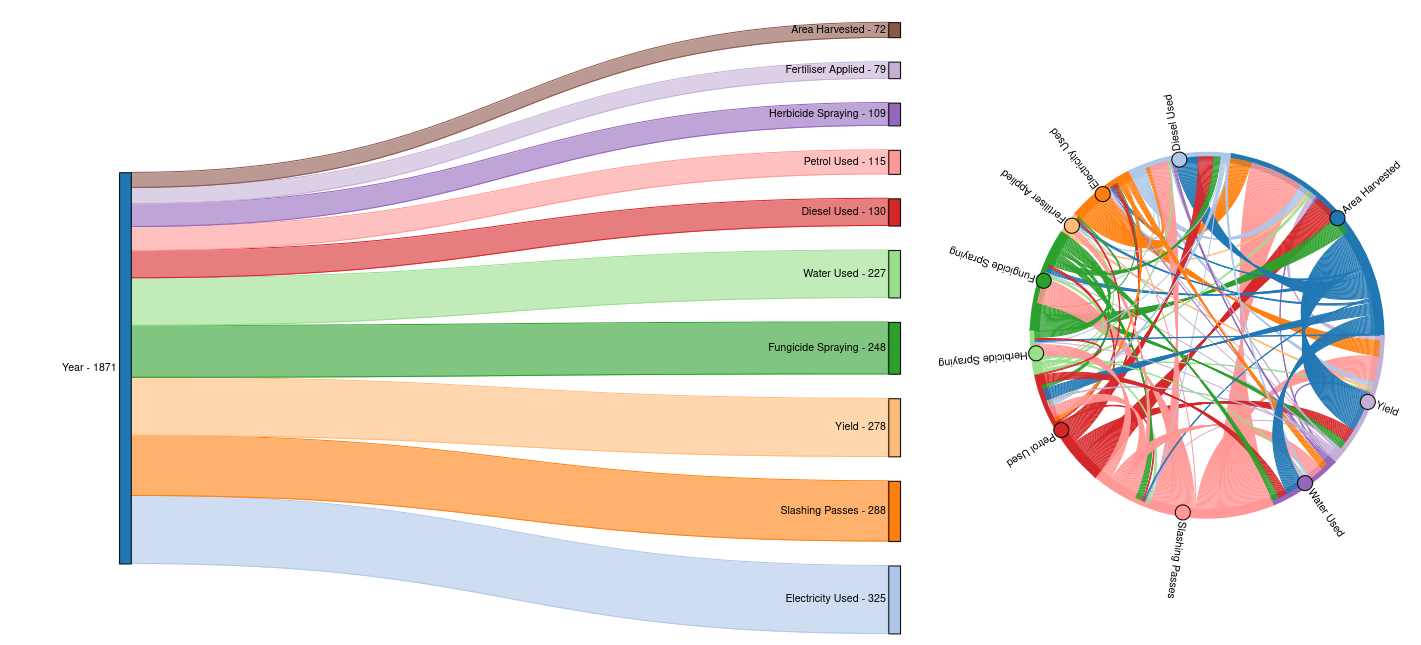
\includegraphics{year.png}}
  \caption{The left-hand side depicts the 10 most important variables in predicting Year using XGBoosted trees as a measure of node occurrence, using a Sankey diagram. The right-hand side depicts the interrelated importance of the ten predictor variables using a chord diagram.}\label{fig:year_sankey}
\end{figure}

\subsection{Operating Costs}

\begin{figure}
  \resizebox{\textwidth}{!}{
  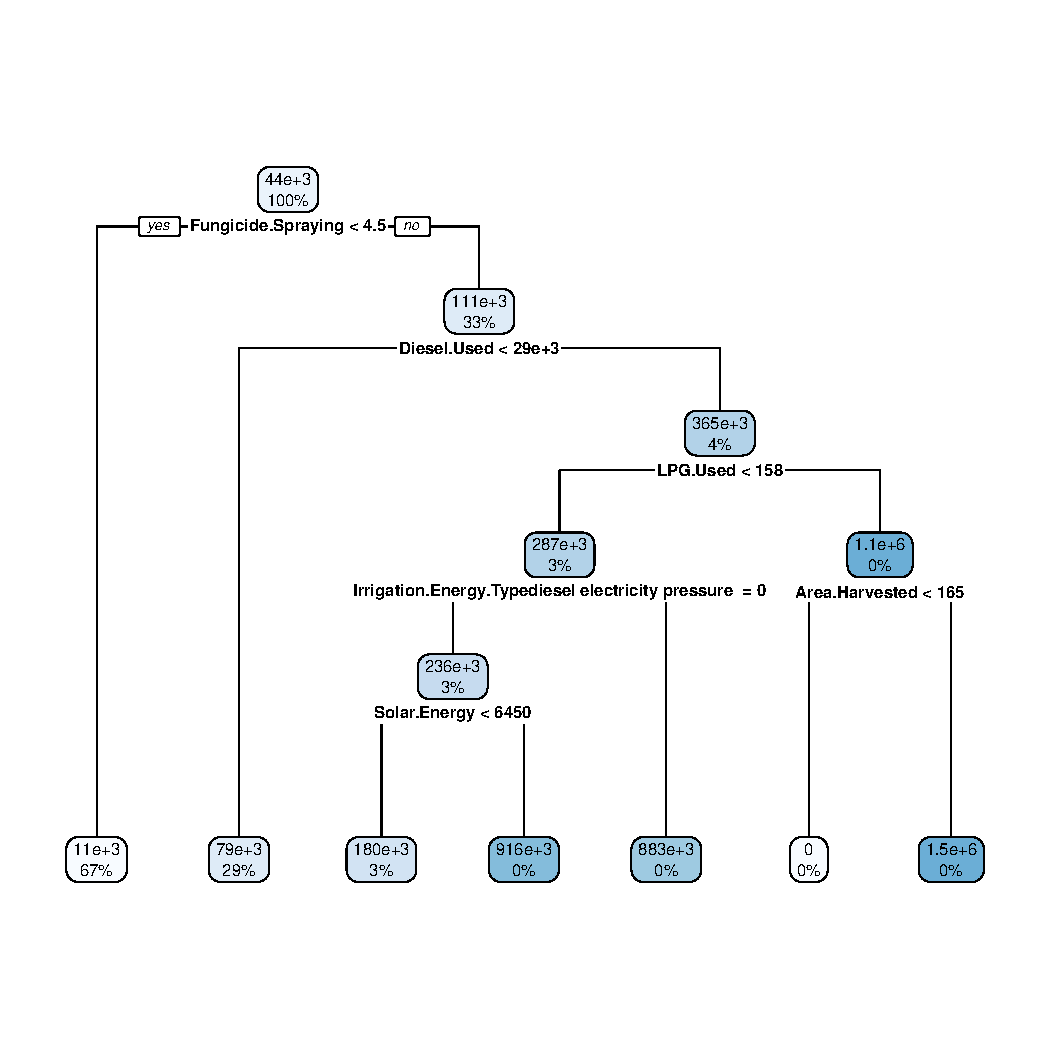
\includegraphics{operating_costs.pdf}}
  \caption{Decision tree predicting Operating Costs. Each node indicates the class predicted, and the proportion of elements agreeing with nodes partitioning, with the left direction indicating a yes to the nodes rule.}\label{fig:operating_costs_tree}
\end{figure}

\begin{figure}
  \resizebox{\textwidth}{!}{
  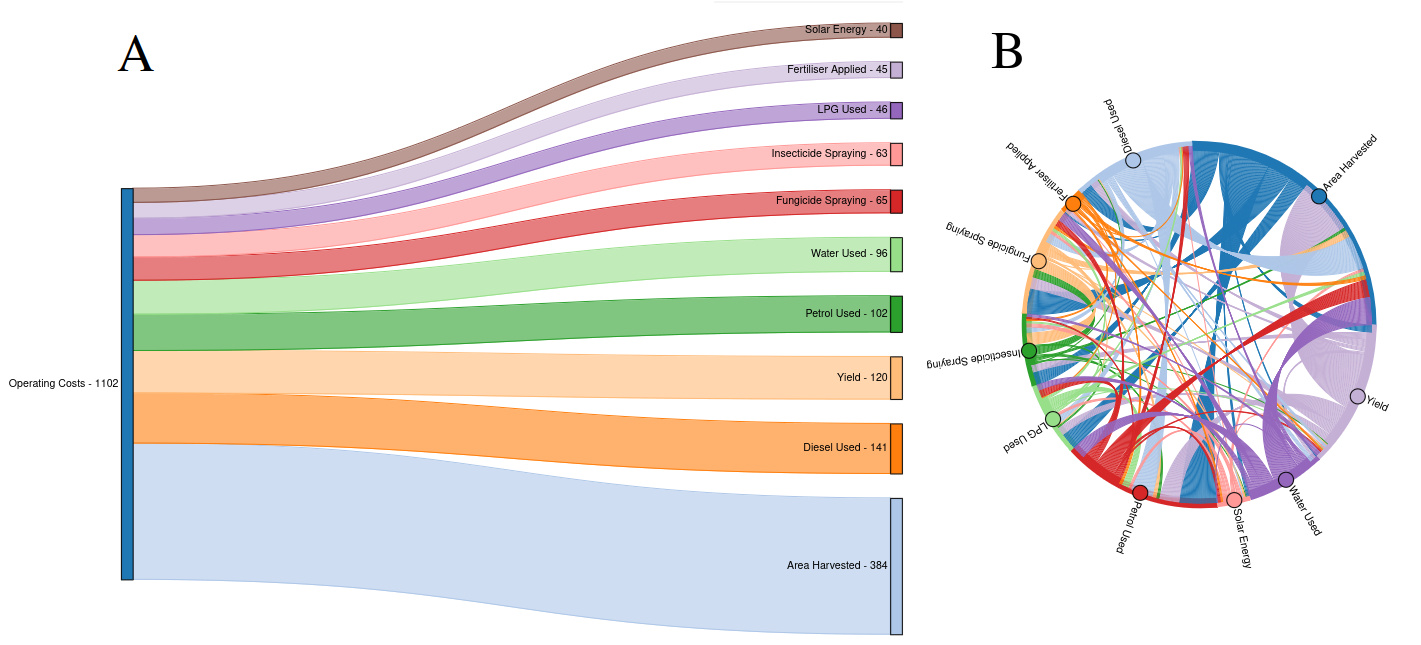
\includegraphics{operating_costs.png}}
  \caption{The left-hand side depicts the 10 most important variables in predicting Operating Costs using XGBoosted trees as a measure of node occurrence, using a Sankey diagram. The right-hand side depicts the interrelated importance of the ten predictor variables using a chord diagram.}\label{fig:operating_costs_sankey}
\end{figure}

\subsection{Profit}

\begin{figure}
  \resizebox{\textwidth}{!}{
  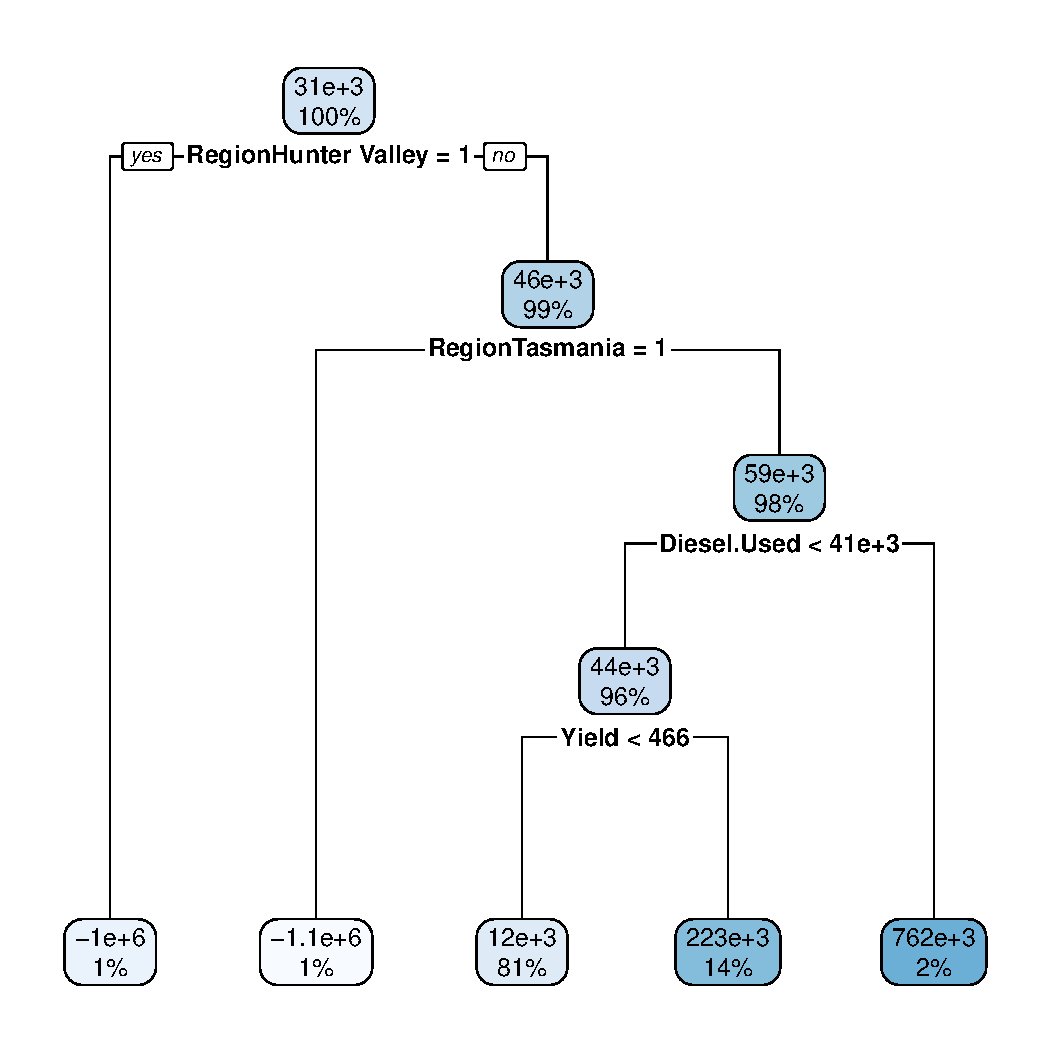
\includegraphics{profit.pdf}}
  \caption{Decision tree predicting Profit. Each node indicates the class predicted, and the proportion of elements agreeing with nodes partitioning, with the left direction indicating a yes to the nodes rule.}\label{fig:profit_tree}
\end{figure}

\begin{figure}
  \resizebox{\textwidth}{!}{
  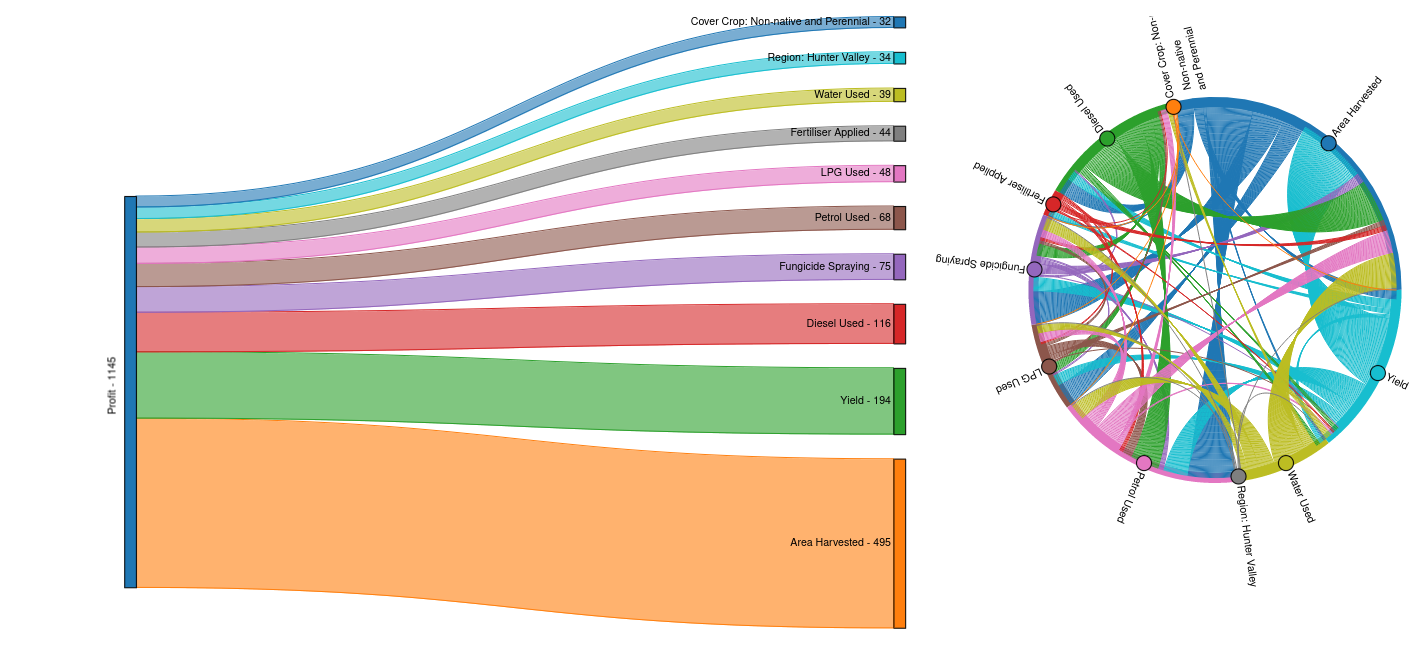
\includegraphics{profit.png}}
  \caption{The left-hand side depicts the 10 most important variables in predicting Profit using XGBoosted trees as a measure of node occurrence, using a Sankey diagram. The right-hand side depicts the interrelated importance of the ten predictor variables using a chord diagram.}\label{fig:profit_sankey}
\end{figure}

\subsection{Validation}

\begin{table}[]
  \caption{Validation and training accuracies of each multiclass variable.}
  \begin{tabular}{@{}ccc@{}}
  \toprule
  \textbf{Variable} & \textbf{Validation} & \textbf{Training} \\ \midrule
  \textbf{cover crops} & 0.364086 & 0.396418 \\
  \textbf{water type} & 0.742097 & 0.928905 \\
  \textbf{profitable} & 0.705882 & 0.719737 \\
  \textbf{irrigation type} & 0.841845 & 0.847554 \\
  \textbf{giregion} & 0.505824 & 0.568242 \\
  \textbf{irrigation energy} & 0.746293 & 0.836405 \\
  \textbf{data year id} & 0.422003 & 0.518059 \\ \bottomrule
  \end{tabular}
  \end{table}



\subsection{Model 1 GI Regions}

The first Model was used to classify GI regions % Interestingly the firs I am hearing of this - each model needs to be more well summarised. A table would be good.
and resulted in an accuracy of 36.48\% across 52 classes. The most prominent features used to classify regions were the types of water resources available (see Figure 1). Two regions, the Riverland and Coonawarra, were the most accurate classes being 92.74\% and 96.97\% respectively.
% it might be worth only talking about the regions that were well classifified - and then talk about their determining traits.
These regions differ greatly in practice and geophysical properties, with the Riverland being a dry warm inland region and Coonawarra being a cooler, wet coastal region. However, they are both similar in operational scales, with vineyards being relatively large compared with other regions.
%Summary statistics regarding these two regions would be a better point of comparison, for example:
%
% How much in size do these operational scales differ?
% How much yield do they differ by?
% What are the differences in rainfall etc
% What makes them unique, different and similar?
%
The differences in resources and practices between these regions are also significant, such as the Riverland utilising the river Murray as a water source.
% What are the specific differences? This is a really critical part of this paper
Many of the regions had significantly lower reporting rates, resulting much poorer classification performance. % This is almost its own paragraph. Why was this case? is it important? what are the similarities and differences of regions that were poorly classified?
 The regions with the most samples performed the best (see Table 1). Notably bordering regions were routinely grouped together and misclassified as the same region, for example the two closest regions to Coonawarra, Padthaway and Wrattonbulley, were misclassified as Coonawarra even though they had 147 and 137 samples respectively. The same case was found for the Murray Darling, with 143 samples, it was misclassified as the Riverland.
 % THis speaks highly to why regions were poorly classified.
These misclassifications are likely due to the incredibly similar regional properties and close proximity these regions have with one another. Other misclassifications were most likely due to lower reporting rates with many regions being under represented.

% \begin{table}[]
%     \caption{Classification accuracy of the most prominent GI Regions.}
%     \label{tab:accuracy}
%     \resizebox{\textwidth}{!}{
%         \begin{tabular}{@{}llll@{}}
%             \toprule
%             \textbf{} & \textbf{Accuracy} & \textbf{Predicted} & \textbf{Actual} \\ \midrule
%             \textbf{Adelaide Hills} & 30.45\% & 95 & 312 \\
%             \textbf{Barossa Valley} & 51.00\% & 205 & 402 \\
%             \textbf{Coonawarra} & 96.97\% & 192 & 198 \\
%             \textbf{Langhorne Creek} & 22.84\% & 53 & 232 \\
%             \textbf{Margaret River} & 78.82\% & 201 & 255 \\
%             \textbf{McLaren Vale} & 52.89\% & 128 & 242 \\
%             \textbf{Riverland} & 92.74\% & 345 &
%         \end{tabular}
%     }
% \end{table}

\subsection{Climate}
Classifying the SWA climatic categorisation of the given regions had better performance than the GI Regions, with ~41.66\% being classified correctly. These categories were divided into 12 climatic classifications with 3 and 4 separate subsets for rainfall and temperature respectively. The decision tree behaved similarly and over classified climates with higher response rates. The results posed an interesting similarity with grape quality classifier, being influenced predominantly by water and area. The use of fungicide to separate regions that were 'Very dry' and 'Damp' can be considered as indicative of the different practices required due to climatic pressure; fungicides being more prominent in cooler regions with greater rainfall due to the higher risk of disease pressure \citep{reynoldsManagingWineQuality2010}. % interesting although not really appropriate for the results section.
 This could also potentially explain the use of contractor tractor use to discern differences in grape quality, where the lack of contractor use to prevent disease could have led to lowered quality of grapes.

% You really need to show every decision tree.

\subsubsection{Rainfall}
The rainfall decision tree showed a greater use of fungicides sprays to discern between damp and very Dry as shown in Figure 4; with the accuracy improving to 62\% but was unable to effectively discern between dry and very dry regions (see Table 3).

\subsubsection{Temperature}
The classification of GI Regions by their temperatures (see Figure 5) showed similarities to the other trees, with a heavy reliance on the types of water resources used as dominant predictors. The use of contractors % This is super important. Talk about this at lengthi nt the discussion. Find more literature on agriculture and the use of contractors as oppose to self managing issues such as weeds.
was again used to differentiate between warm and cool regions, likely being due to disease pressure. The temperature classification tree was only a minor improvement over the regional classification tree, with an accuracy of 49.26\% as shown in the confusion matrix (see Table 4).

\subsection{Model 3 Grape Quality}
The classification of grape quality through its grade % It might even be worth considering this as pseudo grade - or better define it in some of the australian wine journals rose suggested.
had an accuracy of 55.72\% across 5 separate grades. There was a notable issue with the classification of B grade grapes when compared to A and C (see Table 2). % This is actually really interesting.
 The classification tree itself shows similarities to that of classifying regions in Model 1, with the type of water resource used being a prominent determiner. Although not surprising the number of contractor tractor passes is new deciding factor due disease and pests reducing the potential quality of a crop. The prevalence of contractor use is greater in regions such as the Barossa Valley and the McLaren Vale, this could be due to the difference in operational scales, with larger sites being more likely to have ownership of their own equipment for weeding and spraying due to the cost benefit.

\section{Discussion}
The difference between grape quality is most notable between warm inland regions and coastal regions such as the Riverland and Coonawarra, respectively. Grape quality is only described by a singular variable within this study, however in reality it is driven by market demand and subject to  complex forces such as international market pressure, fire, pests and disease \citep{wineaustraliaNationalVintageReport2019,wineaustraliaNationalVintageReport2020,wineaustraliaNationalVintageReport2021,wineaustraliaNationalVintageReport2022,winemakersfederationofaustraliaNationalVintageReport2015,winemakersfederationofaustraliaNationalVintageReport2016,winemakersfederationofaustraliaNationalVintageReport2017,winemakersfederationofaustraliaNationalVintageReport2018} % The original citation included years prior to this dataset just be casreful with this. It is a bit unclear what you are really trying to cite and its relevance. I think it important to chop this up.
The decision trees were able to offer some insights into the factors that influence grape quality and regional contrasts that contribute to different qualities. The most prominent being what readily available resources of each region were, particular the types of water available. % A citation or reference to a study looking at the disparity in wine regions and their resources - or use the data more to describe these regional differences. Is water availability apparent? Do some regions have access to more sohpisticated water sources such as pressurised water etc.
 Heavy water consumption is often linked to the mass production of grapes, % Really? proce it? Where in the results is this really found?? This sounds like a link to your previous paper but you cannot really show this and you do not really produce evidence to support this claim.
 where lower quality grapes are targeted in a quantity over quality strategy. These types of business decisions are unfortunately obfuscated by lack of in-depth data regarding vineyard business plans. 
 % This point is incredibly important but it, itself, is obfuscated by you odd claims that are not supported by facts. Better to talk about how this could improve and the weaknesses than to start spouting unsupported claims.
 Notably the literature shows that there are many complex decisions to be made on the ground depending on many compounding factors that influence both quality and yield \citep{abadCoverCropsViticulture2021,cortezUsingDataMining2009,hallWithinseasonTemporalVariation2011,i.goodwinManagingSoilWater2009,kasimatiPredictingGrapeSugar2022,oliverReviewSoilPhysical2013,srivastavaNondestructiveSensingMethods2018}
 % Woah woah woah
%
 % what are these decisions??? Slow down speed gonzales!! This is really interseteing and important. Discuss it, its the discussion! God damn I want to know and I wrote this!.
 %
%
% This is not all one paragraph surely! There are so many ideas here that should be discussed!
%
% This leads heavily into the next paper and shows that natural progression. Especially in the sense of: if regions have so much influences, what determines ones use of water, fertiliser, etc. And, what determines the success financially, in quality or quantity? How are thes evariables interacting! The next paper is less about predicting and much more about what interacts with what? Where as this paper is about how things change over landscapes and what localised events helpe to determine decisions and their outcomes.
%

 . There are also further differences when comparing winegrowers to other agricultural industries as they are vertically integrated within the wine industry, tying them to secondary and tertiary industries, such as wine production, packaging, transport and sales. This results in unique issues, where on-the-ground choices are influenced by other wine industry's decisions, such as the use of sustainable practices in vineyards to sell in overseas markets; notably these interactions are further complicated by some winegrowers being totally integrated into wine companies, while others are not (Knight et al., 2019). 
% This is an interesting point. However it would be better to include other industries, such as the ones you touch on in your previous chapter. If industries such as Sake are similar - how do their decisions effect the outcomes of rice quality and Sake? A point of comparison and difference would be great here! 
 It is incredibly difficult to attribute external business decisions to produced grape quality but it is important to acknowledge that some growers are contracted to produce grapes of a particular grade; it is difficult to know whether another consumer may have graded the grape quality differently paying more or less for the same grapes given the opportunity to purchase them.
% What are these business decisions? Can you give some examples?
 It is difficult to untangle the contributing factors to the success of winegrowers and the quality of grapes produced without further specifics of choices made through out a season \citep{leileiheFruitYieldPrediction2022}.
% It is difficult yes, but please at least try! Highlight some of these affects, some of these different contributing factors! What did we really learn by doing this? What can someone take away from this and say thank you for? (like Josh said)

\section{Conclusion}

The type and availability of water resources were a major contributing factor when classifying grape quality and region. This was seen in the two most accurately classified regions, Coonawarra and the Riverland, with the Riverland predominantly utilising river water. Furthermore, the study highlighted the influence of water use, fungicide application, and contractor use in differentiating grape quality, climate and region respectively. These models provide insight into the complex dynamics between regional characteristics, sustainable practices, and grape quality in the Australian winegrowing industry. It is important to acknowledge that grape quality is subject to external influences such as market demands and prior established business arrangements. Further in-depth data and understanding are necessary to fully grasp the nuances of decision-making and the interplay of factors impacting grape quality.
% Interesting - the conclusion is actually reasonable, especially considering the disconnection of ideas and models in this paper.

%%%%%%%%%%%%%%%%%%%%%%%%%%%%%%%%%%%%%%%%%%
%%              End Matter              %%
%%%%%%%%%%%%%%%%%%%%%%%%%%%%%%%%%%%%%%%%%%

\bibliography{references} % This points to the references.bib file - the file extention is automatically added.
\bibliographystyle{elsarticle-harv}

%% The Appendices part is started with the command \appendix;
%% appendix sections are then done as normal sections
 \appendix

\end{linenumbers}
  \end{document}
  
\endinput
